
\section{Detector de picos}
\subsection{Diseño}
 El circuito correspondiente al bloque  detector de picos diseñado se representa en la figura \ref{fig:detectorPicos}. \\\\
 
 
Para los diodos se utiliza el modelo $V_{\gamma}$. Este modelo se resume en el cuadro \ref{tabla:diodo}. Ambos diodos son idénticos. 
\begin{table}[htp]
\centering
\caption{Modelo $\gamma$ diodo}
\label{tabla:diodo}
\begin{tabular}{|l|l|l|}
\hline
Estado & Hipótesis   & Verifición        \\ \hline
ON     & $v_D$ = $V_\gamma$ & $i_D$\textgreater0   \\ \hline
OFF    & $i_D$ =0       & $v_D\leq V_\gamma$ \\ \hline
\end{tabular}
\end{table}
 %Los voltajes $V_{\gamma_i}$ de los diodos $D_i$ son iguales y valen $V_ \gamma$.
 \\\\
 La tensión de entrada es de la forma:
 \begin{equation*}
 		v_{in}(t) = Asin(wt) \hspace{0.5cm} \forall t\geq 0
 \end{equation*}
 
 Todas las resistencias $R_j$ son iguales y su valor es $R$
 % Explicar que se analiza de a tramos.
 % revisar explicación de modelo de diodos
\begin{figure}[!htb]
\centering
\begin{tikzpicture}[scale=2]
\draw[color=black, thick][american voltages][american currents]

% NODO A TIERRA
(1,0) node[ground]{}

(1,0) to [R,l=$R_1$] (1,1)

%Amplificador
(2,1.5) node[ op amp ] (opamp) {}
(opamp.out) node[] {}
%----------DIVISOR DE R2 y R1--------------------------- % 
(opamp.+) node[] {}
(opamp.+)-| (1,1)
(1,1.25) to [R,l=$R_2$,*-o](-0.25,1.25)
(-0.25,1.25) node[left] {\Large $v_{in}$}
%-------------------------------------------------------- %
%----------Entrada INVERSORA--------------------------- --% 
(opamp.-) -| (1, 2.75)  to [D*,l_=$D_1$,v^>=$v_{D1}$, i_=$i_{D1}$,*-](3,2.75) |- (opamp.out)
(1,2.5) to (1,3.25) to [R,l=$R_4$](4.5,3.25) to (4.5,1.5)
(-0.25,1.75) to [R,l=$R_3$,-*](1,1.75) 
%----- ------NODO A TIERRA------------------------------- -%
(-0.25,1.75) node[ground, rotate=-90]{}
%--------------------------------------------------------- %
(3,1.5) to [D*,l_=$D_2$, v^>=$v_{D2}$, i_=$i_{D2}$,-*](4.5,1.5)
(4.5,0) to [C,l^=$C$,v_<=\Large $ v_{out}$](4.5,1.5)
% NODO A TIERRA
(4.5,0) node[ground]{}
% ------------- %
(opamp.-) node[above] {\Large $v^-$}
(opamp.+) node[above] {\Large $v^+$}

%---------Fuentes de alimentacion ------------------------- %
(opamp.up) --++ (0,0.1) node[above]{15\,\textnormal{V}}
(opamp.down) --++(0,-0.1) node[below]{-15\,\textnormal{V}}

;
%\draw[black,thick,dashed] (-0.45,1.9) rectangle (3.25,-0.35);

%\draw[black,thick,dashed] (-0.45,4.8) rectangle (3.25,2);
\end{tikzpicture}
\caption{Detector de picos}
\label{fig:detectorPicos}
\end{figure}
\\
Se analiza el circuito en etapas. Se estudia el transitorio con $D_1$ OFF y $D_2$ ON. En régimen, el circuito funciona en dos etapas, intercalándose entre $D_1$ ON y $D_2$ OFF,y $D_1$ OFF y $D_2$ ON. 
\subsubsection{Desde $t=0$ hasta $t=t_1$}
En esta etapa, se supone $D_1$ OFF y $D_2$ ON. Estas suposiciones se traducen en lo expuesto en el cuadro \ref{cuadro:DP1eraEtapa}.


\begin{table}[!htb]
	\centering
	\caption{Hipótesis y condiciones a verificar en primera etapa.}
	\label{cuadro:DP1eraEtapa}
	\begin{tabular}{lll}
		\multicolumn{3}{l}{Desde $t=0$ hasta $t=t_1$}                                                                      \\ \hline
		\multicolumn{1}{|l|}{Diodo} & \multicolumn{1}{l|}{Hipótesis}          & \multicolumn{1}{c|}{Condición a Verificar}             \\ \hline
		\multicolumn{1}{|c|}{$D_1$} & \multicolumn{1}{l|}{$i_{D1}=0$}         & \multicolumn{1}{c|}{$v_{D1}\leq V_\gamma$} \\ \hline
		\multicolumn{1}{|c|}{$D_2$} & \multicolumn{1}{l|}{$v_{D2}= V_\gamma$} & \multicolumn{1}{c|}{$i_{D2}\textless 0$}        \\ \hline
	\end{tabular}
\end{table}

Dado que por hipótesis $i_{D1}=0$, se configura un divisor de tensión entre $R_3$ y $R_4$ de forma tal que:
	$$ v^-=\frac{v_{out}}{2}$$

Además, a causa del divisor de tensión formado por $R_2$ y $R_1$, sabemos que:

$$v^+ = \frac{v_{in}}{2}$$

Por tanto, considerando que hay un cortocircuito virtual ($v^-=v^+$), se tiene:
\begin{equation}
v_{out}(t)= v_{in}(t) \hspace{0.5cm} \forall t\leq t_1
\label{eq:v_{out}}
\end{equation}

Donde $t_1$ es el instante en que deja de cumplirse la condición más restrictiva de las expuestas en el cuadro \ref{cuadro:DP1eraEtapa}.\\\\
{\large \bf Condición para $D_1$:}

Planteando las caídas de tensión en $D_1$, $D_2$ y $C$, tenemos:

$$v_{D1}= v ^- - (v_{D2}+ v_{out})$$

Sabemos que $v_{out}(t)=v_{in}(t)$ y además por hipótesis $v_{D2}=V\gamma$ . Sustituyendo en $v_{D1}$ obtenemos:
$$v_{D1}=-\left(\frac{v_{in}}{2} +V\gamma \right)$$

Imponiendo $v_{D1} \leq V_\gamma $ se obtiene la condición:

\begin{equation}
 v_{in}(t) \geq -4V\gamma 
 \label{eq:d1}
\end{equation}

Suponiendo que $t_1<\frac{\pi}{w}$ se tiene que $v_{in}\geq 0$. Por lo tanto, esta condición se verifica.

{\large \bf Condición para $D_2$:}

Por ley de nodos se tiene que la corriente $i_{D2}$ es la suma de la corriente por el condensador y la corriente por  $R_{4}$. 
Además se impone $i_{D_{2}}>0$. Entonces
\begin{equation*}
      i_{D_{2}} = C \frac{dv_{in}(t)}{dt} + \frac{v_{in}(t)}{2R}  > 0
\end{equation*}

Por lo que se debe verificar
\begin{equation*}
\frac{dv_{in}(t)}{dt} > \frac{-v_{in}(t)}{2RC} \hspace{0.5cm} \Rightarrow Awcos(wt) > \frac{-Asen(wt)}{2RC}
\end{equation*}

\begin{equation*}
2RCw > -tan(wt)
\label{eq:t1}
\end{equation*}

La condición \ref{eq:t1} se verifica mientras $t < \frac{\pi}{2w}$.  Por lo tanto 

\begin{equation}
t_{1} = \frac{\pi}{2w}
\end{equation}

\subsubsection{Desde $t=t_1$ hasta $t=\frac{2\pi}{w}$}

En esta etapa, se supone $D_1$ ON y $D_2$ OFF. Estas suposiciones se traducen en lo expuesto en el cuadro \ref{cuadro:DSegEtapa}.


\begin{table}[htb]
	\centering
	\caption{Hipótesis y condiciones a verificar en segunda etapa.}
	\label{cuadro:DSegEtapa}
	\begin{tabular}{lll}
		\multicolumn{3}{l}{Desde $t=t_1$ hasta $t=\frac{2\pi}{w}$}                                                                      \\ \hline
		\multicolumn{1}{|l|}{Diodo} & \multicolumn{1}{l|}{Hipótesis}          & \multicolumn{1}{c|}{Condición a Verificar}             \\ \hline
		\multicolumn{1}{|c|}{$D_2$} & \multicolumn{1}{l|}{$i_{D2}=0$}         & \multicolumn{1}{c|}{$v_{D2}\leq V_\gamma$} \\ \hline
		\multicolumn{1}{|c|}{$D_1$} & \multicolumn{1}{l|}{$v_{D1}= V_\gamma$} & \multicolumn{1}{c|}{$i_{D1}\geq 0$}        \\ \hline
	\end{tabular}
\end{table}

Al igual que en la parte anterior, se considera un cortocircuito virtual ($v^-=v^+$). Entonces por $R_3$ circula una corriente:
\begin{equation*}
	i_3(t) = \frac{v_{in}(t)}{2R}
\end{equation*}

Al condensador ingresa una corriente de
\begin{equation*}
		i_c(t) = \left( \frac{v_{in}(t)}{2}-v_{c}(t)\right) \frac{1}{R} = C \frac{dv_{c}(t)}{dt}
\end{equation*}

Entonces la corriente que circula por $D_1$ es 

\begin{equation*}
	i_{D1} = - \left( i_c + i_3 \right)
\end{equation*}

Se utiliza la transformada de Laplace para resolver la ecuación diferencial lineal de primer orden:
\begin{equation}
\frac{dv_c(t)}{dt}+\frac{v_c(t)}{RC}=\frac{v_{in}(t)}{2RC}
\end{equation}

Se utilizan las siguientes transformadas:

\begin{equation*}
	L\left[ v_{in}(t) \right] = A\frac{w}{s^2 + w^2}
\end{equation*}


\begin{equation*}
	L \left[ \frac{dv_c(t)}{dt} \right] = sV_c(s)-v_c(t_1)
\end{equation*}

Obteniéndose:

\begin{equation*}
	V_c(s) = \frac{A}{2}\frac{w}{(s^2+w^2)(1+\tau s)} \hspace{0.5cm} + \hspace{0.5cm} \frac{\tau v_c(t_1)}{1+\tau s} \hspace{0.5cm} con \hspace{0.5cm} \tau = RC \hspace{0.5cm} v_c(t_1) = A
\end{equation*}
 Utilizando: 
 
 \begin{equation*}
 L^{-1}\left[ \frac{w}{(s^2+w^2)(1+\tau s)} \right] = \frac{\tau w e^{-\frac{t}{\tau}}}{1 + (\tau w)^2} + \frac{sen(wt-argtan(\tau w)}{\sqrt{1+(\tau w)^2}}
 \end{equation*}
 \begin{equation*}
 	L^{-1}\left[ \frac{1}{1+\tau s}\right] = \frac{e^{\frac{-t}{\tau}}}{\tau }
 \end{equation*}

Al antitransformar se obtiene:

\begin{equation*}
	v_c(t) = A\left(\frac{1}{2}\left[ \frac{\tau w e^{-\frac{t}{\tau}}}{1 + (\tau w)^2} + \frac{sen(wt-argtan(\tau w)}{\sqrt{1+(\tau w)^2}}  \right] + e^\frac{-t}{\tau } \right)
\end{equation*}


\begin{equation*}
	i_{D1} = A \left( \frac{Cw}{2} \left[ \frac{- e^\frac{-t}{\tau}}{1+(\tau w)^2} + \frac{cos(wt-arctan(\tau w))}{\sqrt{1+(\tau w)^2}}\right] -\frac{e^\frac{-t}{\tau}}{\tau}+\frac{sen(wt)}{2R}\right)
\end{equation*}





{\large \bf Condición para $D_1$:}


Se tiene que verificar que $i_{D1}$ es positiva para $t>t_1$

En la figura \ref{fig:id1} se observa el gráfico de la corriente $i_{D1}$ para $t>t_1$. Esta condición se cumple hasta $t_2<\frac{5T}{4}$ con $T = \frac{2\pi}{w} = 0.1ms$. El valor de $t_2$ se obtiene numéricamente. Este es: $t_2 = 0.1221ms$.

\begin{figure}[H]
\centering
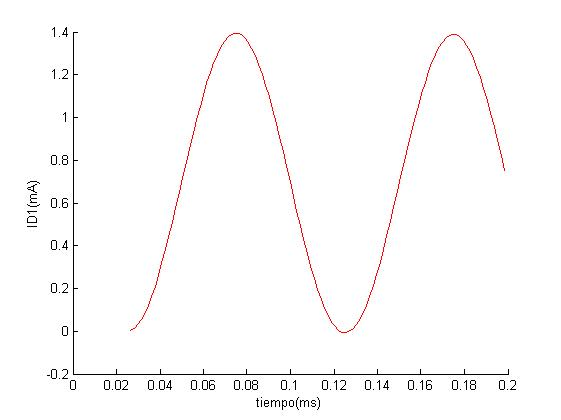
\includegraphics[width=0.6\textwidth]{DetectorDePicos/id1.jpg}
\caption{Corriente por D1}
\label{fig:id1}
\end{figure}

{\large \bf Condición para $D_2$:}

Se tiene que verificar que la tensión en bornes del diodo sea menor a $V_\gamma$. Se tiene
\begin{equation*}
	v_{D2} = v_{amp}-v_c = \frac{v_{in}(t)}{2} - V_\gamma -v_c < V_\gamma
\end{equation*}

\begin{equation*}
	\frac{v_{in}}{2} < v_c+2V_\gamma
\end{equation*}

Dado que $\tau = RC = 10^{-2} > T=10^{-4}$, la descarga del condensador se considera despreciable. Por lo que se verifica la condición ya que $v_c(t=t_1) = A$.\\

Entre $t_2$ y $\frac{5T}{4}$ se vuelve al caso 1.


\subsection{Simulación del circuito en \emph{LTSpice}}

Se simula el circuito con las componentes vistas en el cuadro \ref{tabla:componentesSimuladas} y se gráfica el voltaje $v_{osc}$ en régimen en función del tiempo. La tensión de entrada tiene una amplitud de 7 V y una frecuencia de 10kHz. Dicha gráfica se puede ver en la figura \ref{sim:Vosc}. %INSERTAR SIMULACION.

\begin{table}[htb]
		\tamano\centering
		\caption{Valores de las componentes para la simulación}
		\label{tabla:componentesSimuladas}
		\begin{tabular}{SSSSSSSSS}
			\toprule
			\multicolumn{1}{@{}c@{}}{$R_1$  (\si{\kohm}) } &
			\multicolumn{1}{c}{$R_2$ (\si{\kohm}) } &
			\multicolumn{1}{c}{$R$ (\si{\ohm}) }&
			\multicolumn{1}{c}{$C$(nF) }\\			
			\midrule
			10	& 20	& 120 &  100 \\
			\bottomrule
		\end{tabular}
	\end{table}
El amplificador que se utiliza en la simulación es un TL071 y diodos 1N4148
\begin{figure}[H]
	\centering
	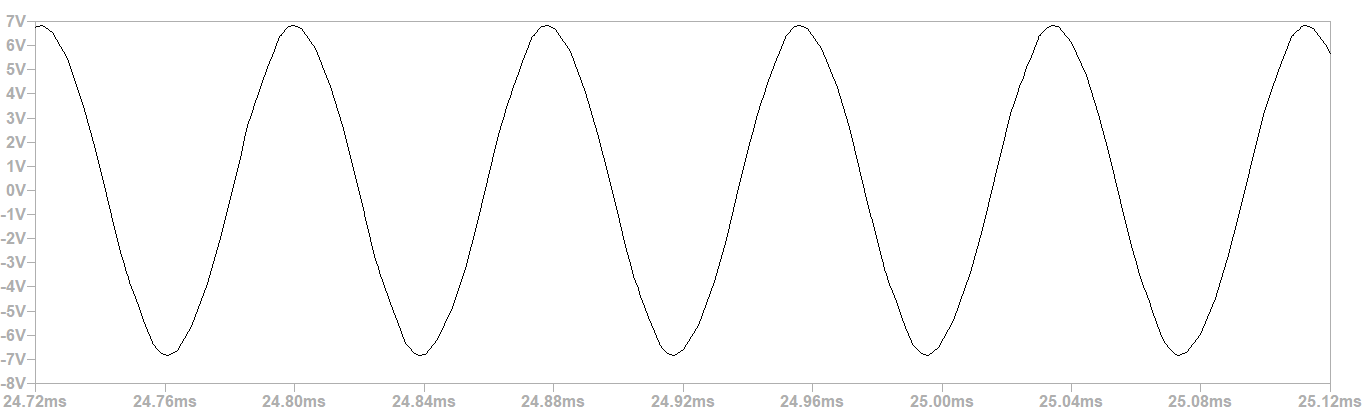
\includegraphics[width=0.6\textwidth]{Oscilador/salida_simulada.png}
	\caption{Simulación: Voltaje de salida del oscilador}
	\label{sim:Vosc}
\end{figure}
\subsection{Implementación (Pendiente)}
VER QUE PASÓ AL IMPLEMENTARLO Y ANOTAR COSAS Y COMPARAR.

\subsection{Amplificador de lm35}
Para medir la temperatura se utilizó un lm35 que da una salida lineal de $10mV/^{o}C$, la temperatura de la leche en la ubre de una vaca ronda los ($35^{o}C$), entonces la salida sera de $350mV$ que es muy bajo y no aprovecha la precisión de la entrada analógica de arduino, por lo tanto se decidió agregar una amplificación no inversora de ganancia $9.33V/V$ donde $R_{6}=10k\Omega$ y $R_{7}=1.2k\Omega$ entonces a $35^{o}C$ se tendrá una salida de $3.27V$.

\section{Cable de señal y alimentación}
Debido a las severas inclemencias que esta sometido el organo de ordeñe (patadas de vacas y caídas), se propuso ubicar el circuito en una zona segura. Por lo tanto se necesitara un cable para transmitir las señales entre las celdas con el circuito y el lm35 con el circuito.\\
El cable ira aferrado al caño de leche que va del organo al caño principal. Encima del caño principal estará ubicado el circuito. Se midió esta distancia ($2.8m$) por lo tanto con un cable de $3m$ es suficiente.\\
Se necesita que el cable tenga como mínimo 5 conductores de señal para las celdas y 3 conductores para el lm35.\\
Se eligió un cable que cuenta con 8 conductores de $0.25mm^{2}$ más un conductor de tierra y una malla de aluminio que protege los conductores de campos electromagnéticos externos.\\
Se procederá a calcular la resistencia de cada conductor. Se sabe que la resistividad del cobre a $25^{o}C$ es $\rho= 17.1\times 10^{-9} \Omega .m$, el largo $l=3m$ y la sección $S=0.25\times 10^{-6}m^{2}$ entonces: \begin{equation}
R_{c}=\dfrac{\rho .l}{S}=0.205 \Omega
\label{eq:RC}
\end{equation}

\section{Testeo del sensor de temperatura}
Como se menciono anteriormente habrá un cable que comunica el lm35 con el amplificador no inversor. Se testeo el funcionamiento de este sistema principalmente para verificar que el cable no afecte el funcionamiento del mismo. Para ello se comparo con una termocupla con una apresiación de $1^{o}C$ FALTA PRESICION Y EXACTITUD. Se Sumergió ambos en agua a diversas temperaturas, a continuación se presentan los resultados.\\



\begin{table}[htp]
\centering
\caption{Comparación sensor con termocupla}
\label{tabla:sensor_temperatura}

\begin{tabular}{|l|l|l|l|}
	\hline
	Termocupla ($^{o}C$) & Sensor ($^{o}C$)  \\ \hline
	43 & 43,3 \\ \hline
    39 & 39,5 \\ \hline
    33 & 34,1 \\ \hline
    31 & 31,8 \\ \hline
    27 & 27,8 \\ \hline
    24 & 25,2 \\ \hline    
\end{tabular}
\end{table}

